% !TeX root = ../thuthesis-example.tex

\chapter{基于多变量互信息的社群层次发现算法}\label{chap:info_clustering}
\section{引言}
在本章中,我们将针对基于图分割的社群发现算法 PSP 效率低的问题,通过
多变量互信息这一度量,引入聚类树的结构,通过结合聚类树的层次特点设计
了新的社群发现算法HPSP。该算法和PSP可以获得相同的层次结构,
但时间复杂度上降低一个数量级。

在提出的HPSP算法基础上,我们进一步研究它的理论性质、
聚类树的数据结构以及HPSP算法在异常值检测领域的应用。

\section{社群发现场景下的多变量互信息理论}
在这一节中,我们首先把\ref{sec:local_geometry}节介绍
的弱独立的概念推广到多个随机变量弱独立,
并在多个随机变量弱独立的条件下,对
\ref{sec:info_clustering}节介绍的多变量互信息
进行化简。
\begin{definition}\label{def:general}
  称$Z_1, \dots, Z_n (n\geq 2)$
  是$\epsilon$-弱独立的,如果存在一个随机变量 $U$
  使得
  $(Z_1, \dots, Z_n)|U$的 概率质量函数 在 $(Z_1, \dots, Z_n)$的
  $\sqrt[n]{\epsilon}$邻域内并且
  $Z_1, \dots Z_n$关于
  $U$的条件分布是独立的。
  \end{definition}
\begin{example}\label{ex:xy_weak_ext}
    考虑例 \ref{ex:Pweak_1}给出的分布,给定$X,Y$
    的分布为$P(x,y)=\frac{1}{4}(1+\epsilon(-1)^{x+y})$。
    我们构造一分布$U$如表所示:
    \begin{table}
      \begin{tabular}{|c|c|c|c|c|}
        \hline
        $P(U=i|X=j, Y=k)$ & $j=0,k=0$ &
        $j=0,k=1$ & $j=1,k=0$  & $j=1,k=1$ \\
        \hline
        $i=0$ & $\frac{(1-\sqrt{\epsilon})^2}{2(1+\epsilon)}$
        & $\frac{1}{2}$ & $\frac{1}{2}$ 
        &  $\frac{(1+\sqrt{\epsilon})^2}{2(1+\epsilon)}$\\
        \hline
        $i=1$ & $\frac{(1+\sqrt{\epsilon})^2}{2(1+\epsilon)}$
        & $\frac{1}{2}$ & $\frac{1}{2}$
        & $\frac{(1-\sqrt{\epsilon})^2}{2(1+\epsilon)}$
        \\
        \hline
      \end{tabular}
    \end{table}

    不难验证$P(X=j, Y=k | U=i)=P(X=j | U=i)
      P(Y=k| U=i)$。此外, $(X, Y)|U=0$
      的概率质量函数 可以写成向量的形式
      $\frac{1}{4}[(1-\sqrt{\epsilon})^2,
      1-\epsilon,
      1-\epsilon,
      (1+\sqrt{\epsilon})^2]$,它在
      $(X,Y)$的概率质量函数 向量
      $\frac{1}{4}[1+\epsilon, 1-\epsilon, 1-\epsilon, 1+\epsilon]$
      的 $\sqrt{\epsilon}$-邻域内。因此
      $X,Y$是$\epsilon$-弱独立的。
\end{example}
例\ref{ex:xy_weak_ext}展示了定义\ref{def:general}和
定义\ref{def:weak_indepedent}在两变量情形的一个共用的例子。
事实上,我们可以证明定义\ref{def:general}是
定义\ref{def:weak_indepedent}的拓展。
\begin{theorem}\label{thm:weak_independence_equivalent}
  如果 对于任何 $x \in \mathcal{X}$,
$Y$关于$X$的条件概率质量函数
$P_{Y|X}(\cdot |x)$在$Y$的$\epsilon$邻域内,那么存在
一个随机变量 $U$
  使得
  $(X, Y)|U$的概率质量函数在 $(X, Y)$的
  $\sqrt{\epsilon}$邻域内并且
  $X, \dots Y$关于
  $U$的条件分布是独立的。
\end{theorem}
\begin{proof}
  由$\epsilon$邻域的定义式\ref{def:eps_neighborhood},
  $P_{Y|X=x}(y) = P_Y(y) + \sqrt{P_Y(y)}\phi_{Y|X=x}(y)
  \epsilon$。定义$\phi_{XY}(x,y)=\sqrt{P_X(x)}\phi_{Y|X=x}(y)$
  则有
  $P_{XY}(x,y) = P_X(x)P_Y(y) + \sqrt{P_X(x)}\sqrt{P_Y(y)}\phi_{XY}(x,y)
  \epsilon$。
  假设$x\in \mathcal{X}$ 且 $y\in \mathcal{Y}$,
  $\mathcal{X}, \mathcal{Y}$ 均为有限的字母集。
  $\phi_{XY}$ 是 $|\mathcal{X}| \times |\mathcal{Y}|$
  的矩阵,其秩为 $r$。可以通过$SVG$分解为
  $\frac{1}{r}\sum_{i=1}^r \phi_i \psi^T_i$,其中$\phi, \psi$
  分别为长度为$|\mathcal{X}|, |\mathcal{Y}|$的
  列向量。构造 $U$ 是$\{1, 2, \dots, 2r\}$ 上面的均匀分布。
  $Z_1, Z_2$ 做如下构造:
  \begin{align*}
    P(Z_1=x|U=i) &= P_X(x) + (-1)^i\sqrt{P_X(x)}\phi_{\lceil i/2 \rceil}(x) \sqrt{\epsilon}, x \in \mathcal{X} \\
    P(Z_2=y|U=i) &= P_Y(y) + (-1)^i\sqrt{P_Y(y)}\psi_{\lceil i/2 \rceil}(y) \sqrt{\epsilon}, y \in \mathcal{Y}\\
  \end{align*}
  $Z_1 | U$ 与$Z_2 | U$ 独立,因此,
  $Z_1, Z_2$ 的联合分布为:
  \begin{align*}
  P(Z_1=x, Z_2=y)& =\sum_{i=1}^{2r}P(U=i)P(Z_1=x|U=i)P(Z_2=y|U=i)\\
  &=P_X(x)P_Y(y) + \sqrt{P_X(x)}\sqrt{P_Y(y)}\frac{\epsilon}{r}
  \sum_{i=1}^{r}\phi_i(x)
  \psi(y) =P(X=x,Y=y)
  \end{align*}
  因此,$Z_1, Z_2$与$X,Y$具有相同的分布。
  不难验证$(Z_1, Z_2)|U$在$(Z_1, Z_2)$的$\sqrt{\epsilon}$邻域内,
  故结论得证。
  \end{proof}
  定理\ref{thm:weak_independence_equivalent}的证明提供了一种生成
  满足弱独立条件的随机变量的方法。即给定均匀分布
  $U$ 在 $n! \times r$个点上取值,
  并且$Z_i|U$在分布$Z_i$的
  $\sqrt[n]{\epsilon}$ 邻域内:
  \begin{equation}
    P(Z_j=z|U=i) = P_{Z_j}(z) + 
    (-1)^{i \,\mathrm{mod}\, n!}\sqrt{P_{Z_j(z)}}
    \phi_{\lceil\, i/n!\, \rceil}(z) \sqrt[n]{\epsilon}, z \in \mathcal{Z_j}
  \end{equation}
  假设$Z_1|U, \dots, Z_n|U$ 独立,可得到
  $(Z_1, \dots, Z_n)|U$的分布。
  不然验证通过这种方法构造出来的分布$Z_1, \dots, Z_n$是弱独立的。

与\ref{sec:info_clustering}节介绍的 PIN 模型类似,
在多个随机变量弱独立的条件下,KL散度的计算可以
与图结构进行对应。即有如下定理:
\begin{theorem}\label{thm:DPX}
若 $Z_1, \dots, Z_n$ $\epsilon$-弱独立, 则有
\begin{equation}\label{eq:PXV}
D(P_{Z_V} || \prod_{C\in \P} P_{Z_{C}}) = {1 \over 2}
\sum_{\substack{(i,j) \not\in C\\ C\in \P}} \norm{B_{ij}}_F^2 + o(\epsilon^2)
\end{equation}
其中 $B_{ij}$ 是 随机变量  $Z_i$ 和 $Z_j$
之间的$B$ 矩阵(参见式\ref{eq:Ixy})而 $\P$是$V$的一个分割(
参见式\ref{eq:IPZV})。 
\end{theorem}
若$ n = 2$,定理\ref{thm:DPX} 即是用 $B$ 矩阵估计互信息,
与 式 \eqref{eq:Ixy} 相同。
因此,定理\ref{thm:DPX}可看成式 \eqref{eq:Ixy} 
的拓展。

定理 \ref{thm:DPX} 是关于弱独立的随机变量的。
现在我们把它拓展到针对数据样本。
给定一 $K$ 个聚类簇的数据集,一共有 $n$ 个样本。
每个 聚类簇被看成一个随机变量。
假设第 $i$ 个 聚类簇 $Z_i$ 字母集 为 $\abs{\mathcal{Z}_i}$,
全局约束是 $\sum_{i=1}^K \abs{\mathcal{Z}_i} = n$。
假设$Z_1, \dots, Z_K$弱独立,
由弱独立的定义式 \ref{def:general}, $Z_i$ 和 $Z_j$ $\epsilon$-弱独立 ($i\neq j$),
于是我们有
\begin{equation}\label{eq:phi_w}
P_{Z_i Z_j}(z_i, z_j) = P_{Z_i}(z_i)P_{Z_j}(z_j) + \epsilon \sqrt{P_{Z_i}(z_i)P_{Z_j}(z_j)} \phi_{Z_i Z_j}(z_i, z_j) + o(\epsilon)
\end{equation}
因此,由 \eqref{eq:Ixy}式,
 $\norm{B_{ij}}_F^2 = \epsilon^2 \sum_{z_r \in \mathcal{Z}_i, z_s \in \mathcal{Z}_j} \phi^2_{Z_i Z_j}(z_r, z_s)$ 
 并且 式 \eqref{eq:PXV} 可以展开成
\begin{equation}\label{eq:PXV_Data}
D(P_{Z_V} || \prod_{C\in \P} P_{Z_{C}}) =
{\epsilon^2\over 2}\sum_{\substack{(i,j) \not\in C\\ C\in \P}}
\sum_{z_r \in \mathcal{Z}_i, z_s \in \mathcal{Z}_j}  \phi^2_{Z_i Z_j}(z_r, z_s) + o(\epsilon^2)
\end{equation}
我们可以把
$\phi^2_{Z_i Z_j}(z_r, z_s)$ 这一项
当成一个有$n$个节点的图的
边的权值。
图的每一个节点对应一个数据点。
为简化符号, 令 $w_{rs} = \phi^2_{Z_{d(z_r)}Z_{d(z_s)}}(z_r, z_s)$
\footnote{当 $d(z_r) = d(z_s)$ 时,
我们仍可以形式化的定义 $w_{rs}$ 为远大于$\max\{\phi^2_{Z_i Z_j}(z_r, z_s), i\neq j\}$
的值。},
其中,$d(z_r)$ 把节点映射到它所属的随机变量的序号, 定义域 为 $1\leq r,s \leq \abs{V}$。
我们也可以展开 每个 $Z_i$ 到它的节点集 并且将分割 $\P$
看成是对节点集的分割。
假设我们考虑的图 $G(V, E)$ 是有向的
\footnote{有向图的假设可以减少计算量而不失一般性},
类似 式 \ref{eq:IP} 我们定义图的入割函数 (in-cut function) $f(C)$ for $C\subseteq V$ as $f(C) = \sum_{i\not\in C, j\in C, (i,j) \in E} w_{ij}$,
它是所有进入$C$的有向边的权值之和。
基于上面定义的符号,表示KL散度的式 \eqref{eq:PXV_Data} 可以写成聚类簇之间边的权值之和
的形式:
\begin{equation}\label{eq:PXV_Data_Simplified}
D(P_{Z_V} || \prod_{C\in \P} P_{Z_{C}}) = \epsilon^2 \sum_{C \in \P} f(C)+ o(\epsilon^2)
\end{equation}
从而我们获得了在多变量弱独立条件下数据聚类的表达式。
由于$\epsilon$是给定的无穷小量,我们更关心$\epsilon^2$
的系数,该系数即与式\eqref{eq:IP}中的$f[\P]$一样,
也在我们求解等价的优化问题式\eqref{eq:hlambda}中出现过。
\section{与数据聚类问题的联系}
\label{sec:data_clustering}
社群发现是输入一张图获得节点所属的类别,而
数据聚类的任务与社群发现相同,但其输入是一个数据矩阵,
其中行数是数据的个数而
每一行的向量代表该数据的特征。二者可以通过
输入数据的格式转换来实现算法互通。一般而言,
从数据矩阵到图的变换是可以通过选取一
相似度度量$d(\cdot,\cdot)$作用到数据上
获得图中边的权值,即$w_{ij}=d(x_i, x_j)$。
在这一节中,
我们研究的重点是如何用
\eqref{eq:hlambda} 实现数据聚类的任务。
在永野清仁的文章中\cite{mac},已经有用RBF核作为相似度度量的
尝试,但局限于该相似度度量在小规模真实世界数据集上表
现不佳,此外相似度度量本身具有一些超参数,也会影响聚类
效果。我们通过使用交叉验证、网格搜索,及对
不同相似度度量的枚举,试图寻找特定问题下具有
较好表现的相似度度量及其超参数。

我们使用5种数据集对基于图分割的数据聚类方法
进行测试,各数据集的基本情况如表\ref{tab:clustering_dataset}
所示。
\begin{table}[!ht]
  \centering
  \begin{tabular}{|c|c|c|c|}
    \toprule
    名称 & 样本数量 & 类别数量 & 特征维度 \\
    \midrule
    Gaussian & 100 & 4 & 2 \\
    Circle & 300 & 3 & 2 \\
    Iris & 150 & 3 & 4 \\
    Glass & 214 & 6 & 9 \\
    Libras & 360 & 15 & 90 \\
    \bottomrule
  \end{tabular}
  \caption{数据聚类测试数据}\label{tab:clustering_dataset}
\end{table}
其中,Gaussian 和 Circle 是人工生成的数据集。
Iris, Glass 和 Libras 是来自 UCI 机器学习标准数据集
\cite{Dua:2019}。

首先我们展示在两个人工生成的数据集上的聚类效果,
Gaussian 数据集的相似度度量取 式\ref{eq:rbf_kernel} 所示的 RBF 核,
$\gamma=0.6$。
\begin{equation}\label{eq:rbf_kernel}
  w_{ij}=\exp(-\gamma ||x_i-x_j||^2)
\end{equation}
Circle 数据集的相似度度量通过 k近邻 进行计算,即仅与自己距离最近的$k$
个数据点有边相连\footnote{所有边权值均为1},取$k=7$。
聚类效果如图 \ref{fig:artificial_dataset_effect} 所示。

\begin{figure}[!ht]
  \begin{subfigure}[b]{\linewidth}
  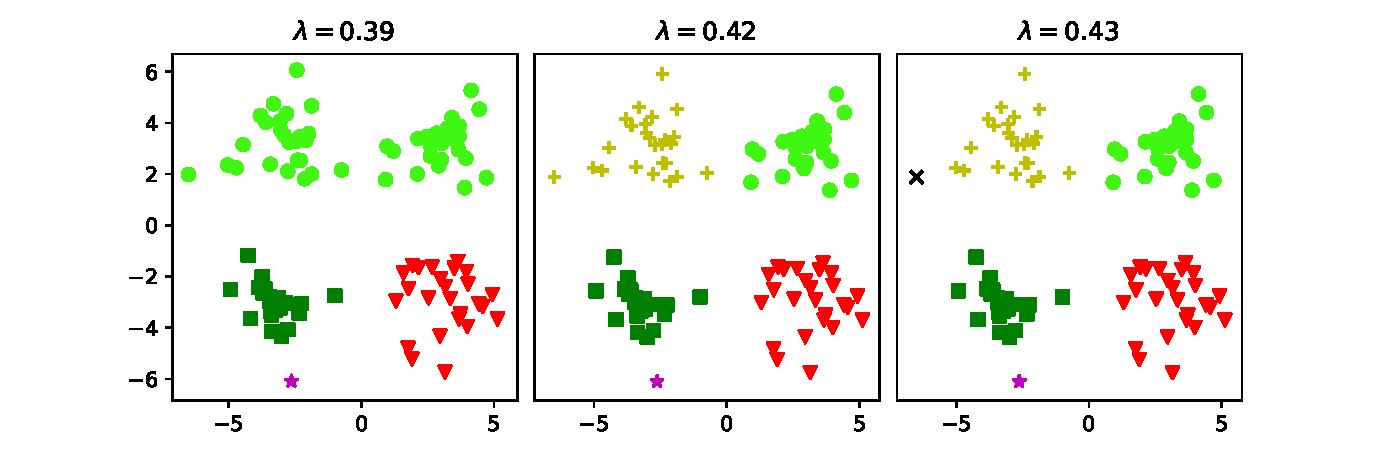
\includegraphics[width=\textwidth]{4part.pdf}
  \caption{有4个类别的 Gaussian 数据集}
  \label{fig:4p}
\end{subfigure}
\begin{subfigure}[b]{\linewidth}
  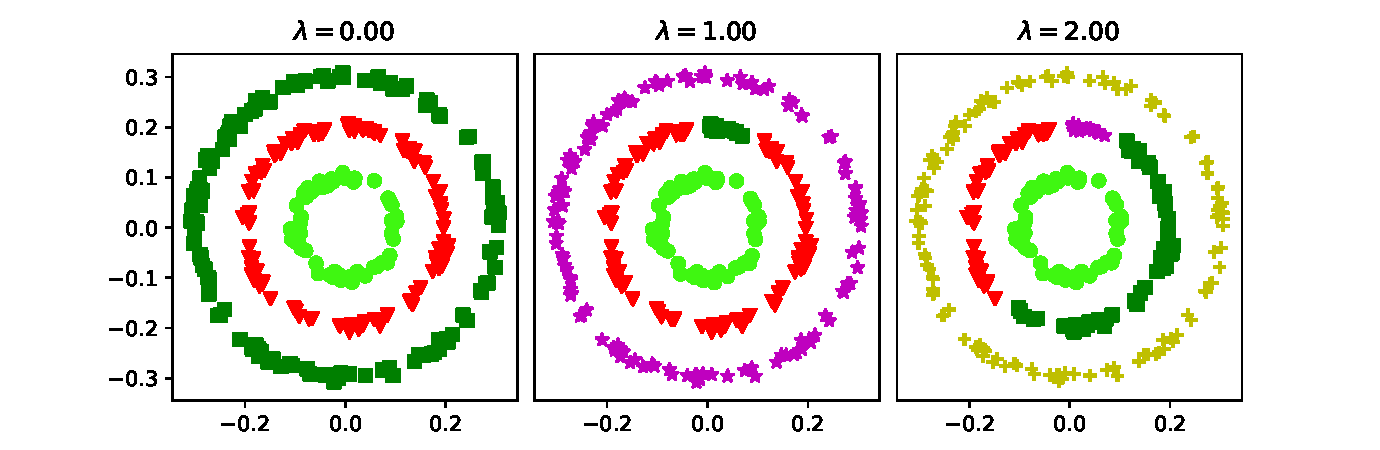
\includegraphics[width=\textwidth]{3circle.pdf}
  \caption{有3个类别的 Circle 数据集}
  \label{fig:3c}
\end{subfigure}
\caption{人工生成的数据集聚类效果}
\label{fig:artificial_dataset_effect}
\end{figure}

从图中可以看到,通过选取适当的阈值 $\lambda$,
可获得与数据的真实类别十分接近的聚类结果,对应于图
\ref{fig:4p} 中的 $\lambda=0.42$
和图\ref{fig:3c} 中的 $\lambda=0.0$。

下面我们在表\ref{tab:clustering_dataset}
的五个数据集上测试比较不同的聚类算法的性能。
我们采用ARI\footnote{adjusted rand index,译为调整兰德系数}
作为衡量指标。该指标介于0到1之间,
其将聚类算法预测的各数据的类别与真实的类别
进行对比,数值越大说明聚类效果越好,等于1说明
两个类别完全一样。我们对比的算法有系统聚类法\cite{slink}、
近邻传播\cite{frey2007clustering}、k-平均算法
\cite{lloyd1982least}
和谱聚类 \cite{shi2000normalized}。
我们通过5轮交叉验证的方式选取各算法的超参数,
表\ref{tab:clustering_dataset}给出了在一定优化空间内
各算法最优的表现,
其对应的超参数详见附表\ref{tab:clustering_alg_hyperparameter}。

从表\ref{tab:clustering_dataset}
可以看出,
信息聚类的方法在 Gaussian, Cirlce, Glass 上表现最好,
在Iris 和 Libras 数据集上的表现不尽人意。
这与文献\citep{mac} 中信息聚类在各数据集上均表现最好的实验结果有出入,
我们由此推测信息聚类可能不适用于真实数据的聚类。

\begin{table}[!ht]
  \centering
\begin{tabular}{lrrrrr}
  \hline
   ARI  &   Gaussian &   Circle &   Iris &   Glass &   Libras \\
  \hline
   系统聚类法         &       1.00 &     1.00 &   0.76 &    0.21 &     0.29 \\
   近邻传播  &       1.00 &     0.14 &   0.19 &    0.19 &     0.23 \\
   信息聚类                  &       1.00 &     0.80 &   0.57 &    0.32 &     0.13 \\
   k-平均算法              &       1.00 &     0.01 &   0.73 &    0.17 &     0.33 \\
   谱聚类   &       1.00 &     0.60 &   0.76 &    0.14 &     0.37 \\
  \hline
\end{tabular}
\caption{聚类算法效果比较}\label{tab:clustering_dataset}
\end{table}

尽管如此, 信息聚类算法在数据的层次聚类上具有明显的优势,
下面我们通过一个实际问题的例子来说明。

为了比较不同的层次聚类方法,最好直接比较聚类树。
为此,
我们使用来自\citet{khan2001classification}的基因表达数据集。
该数据集共有6000多条基因数据,训练集的特征维度是64,
测试集是25。这里我们只使用前300条基因的数据。
由于我们不知道数据的真实聚类树的结构,
我们可以采用分割特征的方法,
分别在两个具有部分特征的数据集上应用聚类算法,
并比较得到的聚类树的相似程度。
这样做的另一个好处是我们还可以测试每种聚类方法的稳定性。

我们将信息聚类算法与基于平均距离度量的系统聚类法、
贝叶斯玫瑰树算法
\cite{blundell2011discovering}
进行了比较。
树的相似性度量是 Robinson-Foulds 距离,
它是将一棵树转换为另一棵树的步骤数
(一个步骤指添加或删除一条边)
\citep{day1985optimal}。
针对不同数据样本数量的实验
结果如图\ref{fig:shc}所示。
可以看出,对于经典的系统聚类方法,
其在不同特征子空间的树的结构相差最大,稳定性较差。
当$n$较大时,信息聚类和贝叶斯玫瑰算法稳定性相当。
但当$n$较小时,信息聚类表现最好。

\begin{figure}[!ht]
\centering
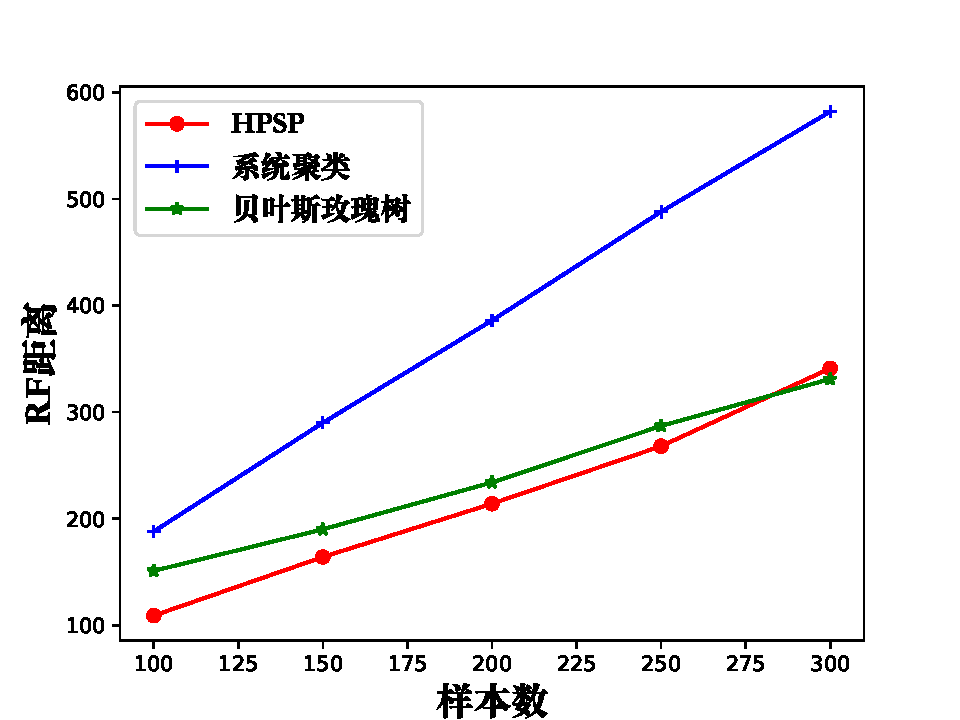
\includegraphics[width=8cm]{plot_results.pdf}
\caption{不同层次聚类算法稳定性的比较}\label{fig:shc}
\end{figure}

\section{社群的层次发现算法}
\label{subsec:cd}
尽管在发现社群的单层结构方面
有很多算法取得了成功,自动发现
复杂网络中的社群层次结构仍是一个困难的问题。
在本节中,我们用实验来证明PSP算法
在恰当定义“边的权重”后,可以成功恢复两层图的层次结构。

对于一个无权图,如果我们简单地把
所有边的权值赋成1,
我们只能得到平凡的聚类树,也即聚类树
只有根节点和叶节点。这个论断可以从如下
定理中得到:
\begin{theorem}\label{thm:triangle}
  在图$G$中,对于没有边相连的两个节点 $w_{ij}=0$。
  并且对于任意三元组$i,j,k \in V$ 权值满足三角不等式 
  $w_{ij} + w_{jk} \geq w_{ki}$,
  则该图的聚类树是平凡的。
\end{theorem}
  
我们通过实验发现使用下述的方法对无权图进行重新
赋权可以达到较理想的效果:
\begin{equation}\label{eq:wij_scheme}
    w_{ij} = 1 + \abs{\{k | (i,k),(j,k) \in E \}} \textrm{ for } (i,j) \in E
\end{equation}
式 \ref{eq:wij_scheme} 对$w_{ij}$
的赋权方法是计算从$i$到$j$不超过两跳的路径数量。

下面我们在一个具有两层结构的图上验证我们的
赋权方法。该数据集在文献
\cite{RN22} 中用于研究动态网络的同步行为,
其结构如图 \ref{fig:c1} 所示。 

\begin{figure}
	\centering
	\begin{subfigure}{0.45\textwidth}
		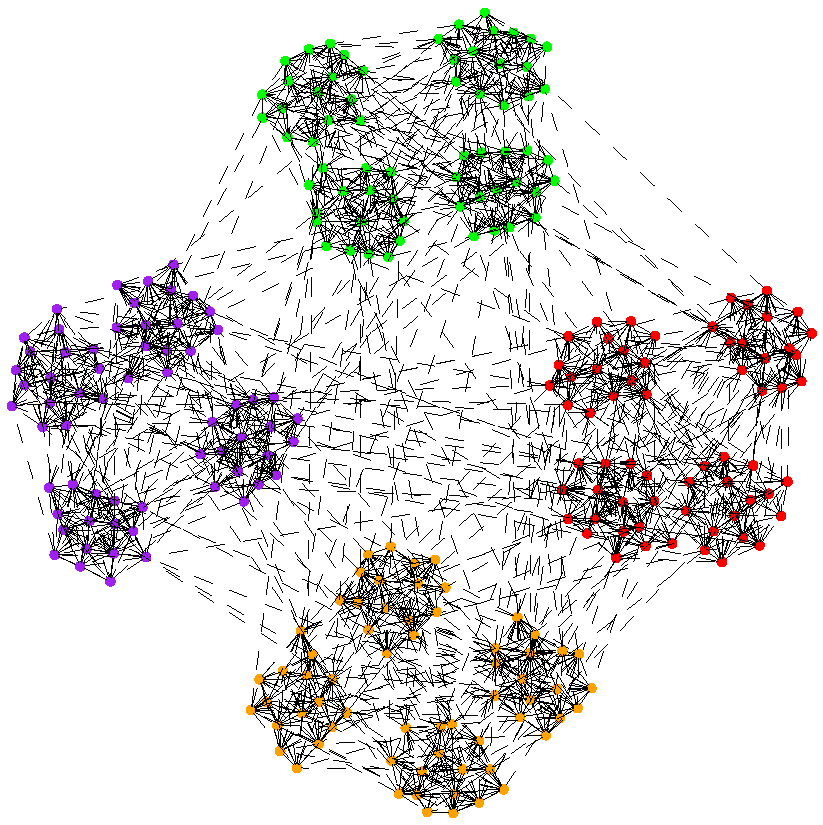
\includegraphics[width=\textwidth]{two_level.pdf}
		\caption{拓扑结构,参数取值为$z_{\mathrm{in}_1} = 14,$ $z_{\mathrm{in}_2} = 3, z_{\mathrm{out}}=1$.}\label{fig:c1}
	\end{subfigure}
	\begin{subfigure}{0.45\textwidth}
		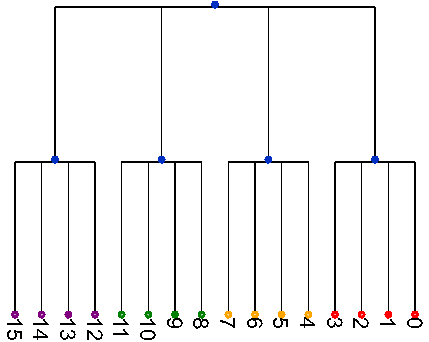
\includegraphics[width=\textwidth]{tree_info-clustering.pdf}
		\caption{聚类树结构,可用PSP算法完全恢复出来。每个叶节点仍包含16个子节点未画出。}
    \label{fig:c2}
	\end{subfigure}
	\caption{具有两层结构的图示意}
\end{figure}

该两层结构的图在宏观层面它包含有 4个 社群,
而每一个中等规模的社群在微观层面又包含4个小社群,
每个小社群有16个节点。
我们用 $z_{\mathrm{in}_1}$ 表示
在小社群内部每个节点连接的边的平均数量;
用 $z_{\mathrm{in}_2}$ 表示
每个大社群内部的中等规模社群之间相互连接的边的平均数量;
用 $z_{\mathrm{out}}$ 表示
不同大社群之间相互连接的边的平均数量。
通过变化参数设定 $\{z_{\mathrm{in}_1}, z_{\mathrm{in}_2}, z_{\mathrm{out}} \}$
我们能得到不同疏密程度的图。

为比较通过算法推断出的聚类树的结构和真实聚类树的区别,
我们使用 归一化的 Robinson-Foulds 距离度量。
它描述了两个具有不同拓扑结构的树之间的距离,
其取值在$[0,1]$ 之间。
我们将基于图的信息聚类算法与
GN (Girvan-Newman 算法) 和 BHCD (一种贝叶斯层次聚类算法\cite{RN23})。
比较的结果如图 \ref{fig:cdr} 所示。
从图 \ref{fig:cdr}中可以看到,在三种不同的参数配置下,
通过基于图的信息聚类算法相比其他方法 可以获得
与真实聚类树更相似的聚类树结构。

\begin{figure}
	\centering
	\begin{subfigure}{0.33\textwidth}
		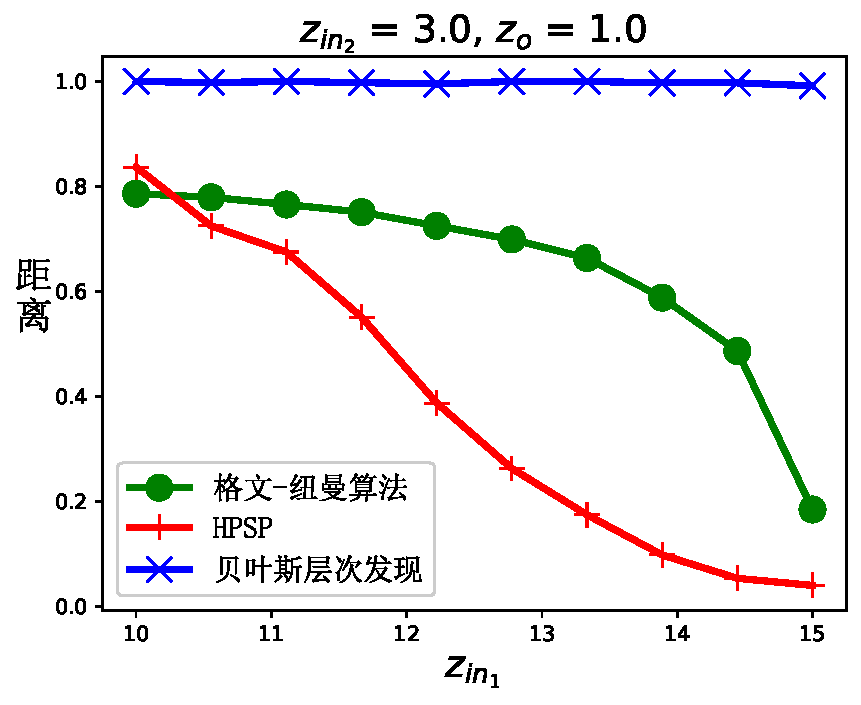
\includegraphics[width=\textwidth]{z_in_1.pdf}
		\caption{}
	\end{subfigure}~
	\begin{subfigure}{0.33\textwidth}
		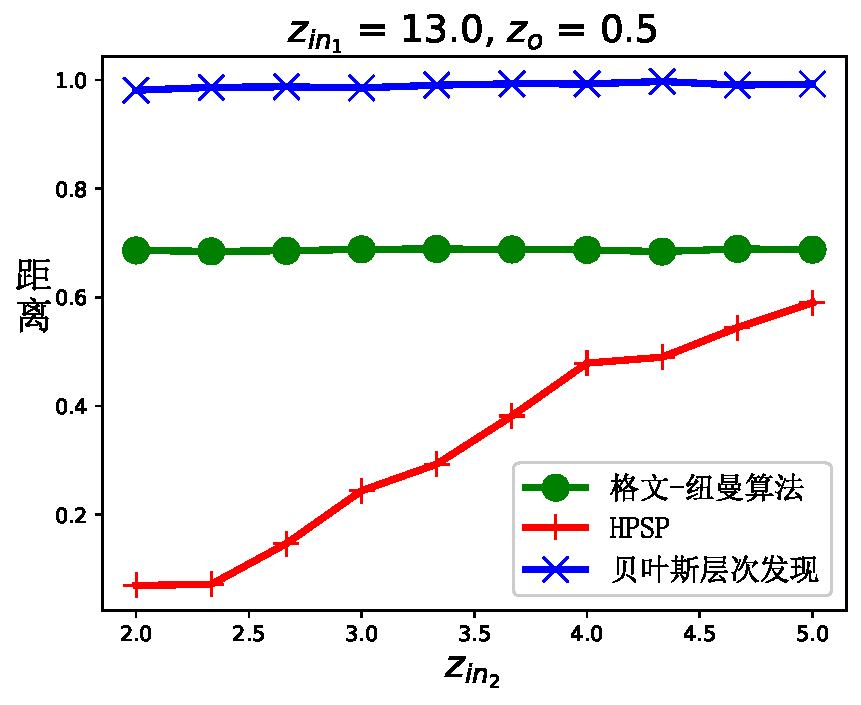
\includegraphics[width=\textwidth]{z_in_2.pdf}
		\caption{}
	\end{subfigure}~
	\begin{subfigure}{0.33\textwidth}
		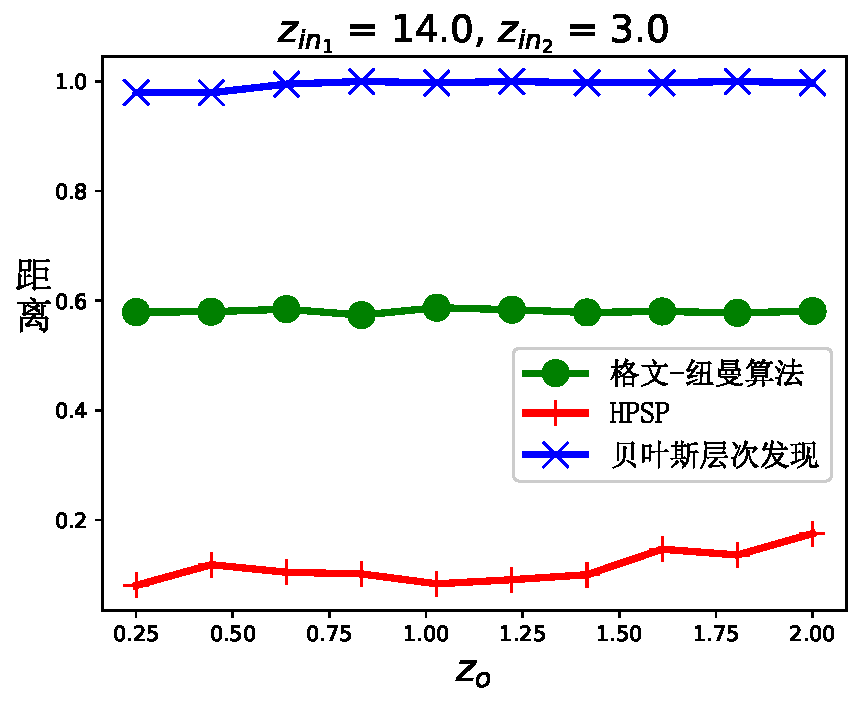
\includegraphics[width=\textwidth]{z_o.pdf}
		\caption{}
	\end{subfigure}
	\caption{不同层次社群发现算法的性能比较。
  更小的距离意味着与真实的聚类树更相似的结构。
  }\label{fig:cdr}	
\end{figure}

\section{基于图分割的社群发现算法及其改进}
在本节中,我们首先介绍我们对PSP算法的改进,并在一定
的假设下证明其理论复杂度,最后比较求解图分割的三种不同实现下
的算法效率。
\subsection{HPSP算法}
我们改进的PSP算法仍将使用
算法 \ref{alg:psp} 中提到的
\texttt{DT} 子函数。
在算法\ref{alg:psp} 中,我们观察到
每次调用 \texttt{DT} 是相互独立的,
并没有利用到聚类树的 固有性质。
如果聚类树的嵌套性质可以被考虑进来的话, 
我们可以在后面的计算中
仅在子图上进行 \texttt{DT} 的调用,
从而可以实现计算效率比PSP算法提升一个数量级。

在给出算法描述之前,我们先定义两个对图的操作:
图限制(restriction)和图收缩(contraction)。
我们称把图$G$限制到集合$C\subseteq V$是指
考虑$G$的节点集为$C$而边的集合为$\{(i,j) \in E | i,j \in C \}$
的子图,
记为$G[C]$。给定$V$的分割 $\P=(C_1, \dots, C_k)$,
图根据$\P$收缩得到一个新的图,其节点集为
$\P$,即第$i$个节点对应$C_i$。边的集合为$\{(i,j) \in [k] | w(C_i, C_j) > 0 \}$。
其中$w(C_i, C_j)=\sum_{r \in C_i, s \in C_j} w_{rs} $
也是新图节点$C_i$和 $C_j$之间的权重。我们把收缩后的图记为
$G[\P]$。


在我们设计的算法中,
假设我们第一次调用DT后得到了
$\P_i = \{C_1, \dots, C_t\}$。
然后我们 分别对每个
$G[C_i](i=1,\dots, t)$
计算 PSP分割。
并从子图的计算中构造 $P_j(j>i)$。
对于 $\P_j(j<i)$,
我们对收缩后的图 $G[\P_i]$ 计算 PSP 分割
可以得到  $P_j(j<i)$ 的结果。
我们把我们的改进方法称为 HPSP,其中 H 表示 “层次的”
英文首字母\footnote{hierarchical},
其描述在算法\ref{alg:psp_i_simplified}中给出。

\begin{algorithm}[!ht]
	\caption{改进的求解主分割序列的算法}\label{alg:psp_i_simplified}
	\begin{algorithmic}[1]
		\REQUIRE 有向图 $G(V, E)$; 边的权值函数 $w(e)$,其中 $e\in E$
		\ENSURE 聚类树 $\mathcal{T}(K, E)$ 其中 $K \subseteq 2^{V}$ 表示节点集
    而 $E$ 表示边的集合。
		\STATE 初始化 树 $\mathcal{T}$:
     $V$ 是根节点,
     $\{j\}(j \in V)$ 是诸叶节点,
     无其他节点。
		\STATE \texttt{Split}($G$)
		\FUNCTION{\texttt{Split}($G$)}
		\STATE $w$ 是 $G$ 所有边的权值之和。
		\STATE $\gamma' = \frac{w}{\abs{V(G)}-1}$
    其中 $V(G)$ 是 图$G$
    的节点集。
    \label{alg:gamma_apostrophe}
		\STATE $(\tilde{h}, \P')
    = \texttt{DT}(G, \gamma')$ 其中
    $\P'$ 是在 式 \eqref{eq:hlambda} 中达到
    最小值 $h(\gamma')$的分割
    并且 $\tilde{h}$ 是对应的最小值。 \label{line:DT}
		\IF{$\tilde{h} = - \gamma'$}
		\STATE 在聚类树
    $\mathcal{T}$ 中把权值 $\gamma'$ 标记在从 $V(G)$ 出发
    到其所有子节点的边上。
		\ELSE
		\FOR{$S$ in $P'$ and $\abs{S}>1$}
		\STATE 在聚类树
    $\mathcal{T}$ 中构造新的节点$s=S$,
    并修改 $S$中元素的父亲节点 为$s$,
    而$s$的父节点为$V(G)$。
		\STATE \texttt{Split}($G[S]$) \label{line:SplitDown}
    %其中 $\widetilde{G}[S]$ 是 $\widetilde{G}$ 限制在 $S$
    %上的子图。
		%\STATE 在 $\widetilde{G}$ 中将 $S$ 缩成一个节点。 % graph \widetilde{G} is modified
		\ENDFOR 
		\STATE \texttt{Split}($G[\P']$)		\label{line:SplitUp}
		\ENDIF
		\ENDFUNCTION
	\end{algorithmic}
\end{algorithm}

\begin{figure}[!ht]
	\centering
	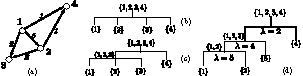
\includegraphics[width=10cm]{alg_illustration.pdf}
	\caption{HPSP 求解图(a)的主分割序列,聚类树经(b), (c) 演化到 (d) }\label{fig:alg_eg}
\end{figure}

\begin{example}
	我们用一个简单的例子来说明
  算法 \ref{alg:psp_i_simplified}。
  考虑图 $G(V, E)$,有 $V=\{1,2,3,4\}, E=\{(1,2),(1,3),(2,3),(1,4),(2,4)\}$。
  边的权值为 $w_{13}=2, w_{12}=5, w_{23}=2, w_{14}=1, w_{24}=1$。
	图 \ref{fig:alg_eg} (a) 中画出了 $G$
  的结构。
  最初的聚类树结构如图 \ref{fig:alg_eg} (b)
  所示。
  根据 
  算法 \ref{alg:psp_i_simplified} 的
  第\ref {alg:gamma_apostrophe}行,
  我们计算 $\gamma' = \frac{11}{4-1}, \tilde{h} = -\frac{16}{3} < -\gamma' $
  且 $\P' = \{\{1,2,3\},\{4\}\}$,
  于是我们得到如图\ref{fig:alg_eg} (c) 所示
  的聚类树结构。
	
	然后我们在 子图 $G[\{1,2,3\}]$ 上运行 PSP 算法,
  $\gamma' = \frac{9}{2}, \tilde{h} = -5 < -\gamma'$
  并且 $\P= \{\{1,2\},\{3\}\}$。 
  于是我们得到了最终的聚类树结构。
  其余的计算给出了聚类树剩余的边的权值,如
  图 \ref{fig:alg_eg} (d) 所示。
\end{example}	
\subsection{时间复杂度分析}

本小节我们分析上小节提出的 HPSP算法 (算法 \ref{alg:psp_i_simplified})的时间复杂度。
首次说明一些惯用语,我们称图是稠密,如果它的边的数量是$n^2$的量级。
也即 $\abs{V} = n, \abs{E} = O(n^2)$。对于稠密的图,由于最大流算法中需要多次遍历
边,会增大时间开销。一般PSP算法复杂度分析即针对最坏的情形,即稠密的图进行。
我们已知的结论有 \texttt{DT} 算法(算法\ref{alg:dt})
的时间复杂度是 $O(n^4)$, 而 PSP算法(\ref{alg:psp})的 
时间复杂度是 $O(n^5)$ \citep{pin}。

我们使用 $T(n)$ 来代表 
\texttt{Split} 函数调用的
时间复杂度。
从算法 \ref{alg:psp_i_simplified} 中可知,
$T(n)$ 的递推关系式为
\begin{equation}\label{eq:Tn}
T(n) = \max \{ C n^4 + \sum_{i=1}^k T(n_i) +
T(k)\delta_{k<n} |
\sum_{i=1}^k n_i = n, n_i \in \mathbb{Z}_{+} \}
\end{equation}
在 式\eqref{eq:Tn} 中,
$Cn^4$ 代表 \texttt{DT} 的时间复杂度。
$\delta_{k<n} = 1$ 是 指示函数,当满足条件 $k<n$时取值为1,
否则 $\delta_{k<n}=0$。
针对 $T(n)$,我们有如下定理:
\begin{theorem}\label{thm:alg_complexity}
	 若 $n_i \leq \frac{n}{2}, \textrm{ for } i=1,\dots,k$ 并且
   $ k \leq \frac{n}{2}$  在式 \eqref{eq:Tn} 中成立, 
   则 $T(n) = O(n^4)$.
\end{theorem}

定理 \ref{thm:alg_complexity} 所要求的条件
限制了聚类树的结构。
它指出,若对于每个非叶节点,其后代数都不超过 $\frac{n}{2}$,则HPSP
算法的时间复杂度是  $O(n^4)$。
该条件适用于很多聚类树的情形,即使有个别节点不满足其假设,$T(n) = O(n^4)$也成立。
我们在保证有相同计算结果的前提下,
提出的HPSP 的时间复杂度的结果要比
PSP算法 \ref{alg:psp} 的$O(n^5)$ 的结果快一个数量级。

即使是最坏的情况,也即,聚类树的深度达到了 $O(n)$ 的数量级。
则\texttt{DT} 不可避免地要调 用 $O(n)$ 次。
在这种情形下,
$T(n)$ 的复杂度的上界是 $C(3^4+4^4 + \dots + n^4) \sim \frac{1}{5}Cn^5$,
其比 算法 \ref{alg:psp} 的结果
快 $5$ 倍。
\subsection{聚类树的数据结构}
在层次聚类中聚类树一般使用关联矩阵(linkage matrix)构造聚类树
\cite{D2011Modern},但这种方法
仅限于一次聚合两个节点的场景。
在允许一次聚合多个节点的情形下,可以使用带权的并查集(weighted Union-Find set)的方法自底
向上构造聚类树
\cite{chan2020agglomerative}。 
但由于我们设计的HPSP算法是
自底向上和自顶向下的混合,不能照搬关联矩阵和并查集的数据结构,而是要结合
HPSP算法~\ref{alg:psp_i_simplified} 的特点重新设计。
为此,
我们采用选取代表元素来构造聚类树,比如对于
聚类树的中间节点$\{1,2\}$选取较小的元素1来代表。
这样做的另一优势是在存储方面,我们无需为中间节点额外开辟空间。
我们采用父节点数组$K$来储存树的结构,而和聚类树边权重相关的数据
用另一数组$W$储存。聚类树的空间复杂度为$2|V|$。
基于以上数据结构,HPSP算法~\ref{alg:psp_i_simplified} 
使用静态数组的实现如算法
~\ref{alg:psp_i_simplified_tree_array} 所示。

\begin{algorithm}[!ht]
	\caption{聚类树的数组实现}\label{alg:psp_i_simplified_tree_array}
	\begin{algorithmic}[1]
		\REQUIRE 有向图 $G(V, E)$; $V=[n]$,边的权值函数 $w(e)$,其中 $e\in E$
		\ENSURE 聚类树 $\mathcal{T}=(K, W)$, $K,W$ 为动态数组,
    $K[i]$ 表示树中节点$i$的父节点的ID,$W[i]$表示节点$i$到其父节点的权值
		\STATE 初始化 $n$ 长的数组 $\mathcal{T}$
     和$W$。
		\STATE \texttt{Split}($G, 1$)
		\FUNCTION{\texttt{Split}($G, s$)}
		\STATE $w$ 是 $G$ 所有边的权值之和。
		\STATE $\gamma' = \frac{w}{\abs{V(G)}-1}$
    其中 $V(G)$ 是 图$G$
    的节点集。
		\STATE $(\tilde{h}, \P')
    = \texttt{DT}(G, \gamma')$ 
		\IF{$\tilde{h} = - \gamma'$}
		\STATE $W[i]=\gamma'$ for $ i \in V(G)$
    \STATE $K[i]=s$ for $i\in V(G)$
    \ELSE
		\FOR{$S$ in $P'$ and $\abs{S}>1$}
		\STATE \texttt{Split}($G[S], j$),其中$j$为$S$中最小的元素
		\STATE $G=$\texttt{Contract}($G, S, j$) \label{alg:contract}
    \ENDFOR 
		\STATE \texttt{Split}($G, s$)
		\ENDIF
		\ENDFUNCTION
	\end{algorithmic}
\end{algorithm}

为标记聚类树中每个节点的父节点,
我们在算法\ref{alg:psp_i_simplified_tree_array}
的 \texttt{Split} 函数中增加了
一个参数$s$,$s$是当前所操作的图中所有节点序号最小的,
对应到聚类树中这些节点的父节点ID。

在第\ref{alg:contract}行的\texttt{contract}函数 是在图$G$中
将$S$中的各节点缩为一个点$j$,边的权值也做相应的调整。
为了提升算法运行效率,和图限制$G[S]$类似,我们可以避免构建新图的操作,
而是直接在原图$G$上进行修改。

另外,从构造好的聚类树中获取正确的分割也是
我们要考虑的问题。
陈聪曾采用一种类似深度优先搜索的策略在聚合的过程中逐步获取分割
\cite{chan2020agglomerative}。
由于我们未存储子节点的信息,因此我们在
获取分割的实现策略上需要另辟蹊径。
为此,我们采用自底向上的方法获取全部的分割,
具体实现见算法~\ref{alg:get_psp}。

\begin{algorithm}[!ht]
	\caption{从聚类树获取主分割序列}\label{alg:get_psp}
	\begin{algorithmic}[1]
		\REQUIRE 聚类树 $\mathcal{T}=(K, W)$
		\ENSURE 序列 $L=[\lambda_1, \dots, \lambda_k]$
    和 $\mathcal{Q}=[\P_0, \dots, \P_k]$.
    \STATE 初始化 $Q\leftarrow \{ \{\{i\}|i\in [n]\} \}, C\leftarrow [n]$ 与哈希字典 $D$,$D$把不存在的键值映射到空集
    \WHILE{$|C|>1$}
		\STATE $(\P,\gamma, C)$ \leftarrow \texttt{Merge}($C$)
    \STATE prepend $P$ to $Q$ and prepend $\gamma$ to $L$
    \ENDWHILE
		\FUNCTION{\texttt{Merge}($C$)}
    \STATE $\gamma = \max_{i\in C} W[i]$
    \STATE $D[k] = \{ j\in C | K[j] = k, W[j]=\gamma\} \cup \{k\} \cup D[k]$
    \FOR{ any $ j \in D[k]$}
    \STATE $D[k] \leftarrow D[j] \cup D[k]$, 并从$D$中删除键值$j$ 
    \ENDFOR
    \STATE $C' \leftarrow  \{j\in C | W[j]<\gamma\}$
    \STATE $\P=\{D[k] | k \in \texttt{key}(D)\} \cup \{\{i\} | i \in [n]\backslash \cup_{k \in \texttt{key}(D)} D[k] \}$
    \RETURN $(\P, \gamma, C')$
		\ENDFUNCTION
	\end{algorithmic}
\end{algorithm}

在算法算法~\ref{alg:get_psp}中,我们
使用了额外的数组$C$来表示合并后当前
剩余的节点,字典$D$储存了如何把剩余的节点展开成聚类簇
的信息。由于\texttt{Merge} 函数最坏调用$n$次,
而计算$\gamma$的时间复杂度是$O(n)$,其它操作不超过$O(n)$,
因此整个转换算法的时间复杂度是$O(n^2)$,相比
定理\ref{thm:alg_complexity}
中给出的$HPHP$ 的$O(n^4)$的时间复杂度,转换本身的时间开销
可忽略不计。

\subsection{代码实现}
尽管最大流算法包比较多,但我们尚未发现
求解层次分割(式\eqref{eq:PSP_structure})的开源实现。
因此我们使用 C++ 实现了跨平台的PSP算法\ref{alg:psp}
(内嵌迪尔沃思截断算法\ref{alg:dt}),并且
我们提供了Python编程语言的接口函数,并在 \url{pypi.org}
平台上以 pspartition
的名字发布,以供后面的研究者使用。
我们的实现使用 CMake 编译,依赖于第三方库 LEMON \cite{dezsHo2011lemon}。 
LEMON 库在我们的算法包中用于构建所需的图数据结构和最大流算法。
这里顺便提及的一点是 LEMON 库里使用的
最大流算法是基于最大标签选择策略的前置推送-标签重贴算法。
根据文献\citet{ahuja1997computational}的比较,该算法
的效率比起其他解最大流问题的算法有明显的优势。

在Python的接口函数方面,我们采用了CPython
跨语言编程的方式,将由 NetworkX \cite{SciPyProceedings_11} 构建的图
转换成用边表示的图传递到C++中的类构造函数中,
计算完成后再把C++中的集合转换成Python中的列表
进行返回。用于求解例 \ref{ex:psp}
的示例 Python 代码如下。
\begin{lstlisting}[language=Python]
  from pspartition import PsPartition
  a = [[0,1,1], [0,2,5], [1,2,1]] #graph edge list,(i,j,weight)
  p = PsPartition(3, a) #3 nodes
  p.run()
  cv = p.get_critical_values() #[2,5]
  pl = p.get_partitions()#[[{0,1,2}],[{0,2},{1}],[{0},{1},{2}]]
\end{lstlisting}

\subsection{不同PSP算法的效率比较}
在本节中,我们将比较 HPSP 算法和PSP算法
(算法\ref{alg:psp})
以及基于参数最大流改进方法\cite{kolmogorov}
的运行效率。我们使用两种不同的数据集,图的边具有不同的
稠密程度。

第一个数据集叫做 Gaussian-blobs,
类似\ref{sec:data_clustering}
节的 Gaussian 数据集,它也是由
4个相同大小的高斯块组成,但我们可以改变
每个块的样本数量。由于我们使用式\ref{eq:rbf_kernel}
计算图中边的权值,边的数量满足 $|E|=\Theta(|V|^2)$。
这里$\Theta$表示$|E|$与$|V|^2$量阶相同。
\newglossaryentry{not:fntheta}
{
  type=notation,
  name={$f(n)=\Theta(g(n))$},
  description={当$n\to \infty$时,$f(n)$和$g(n)$ 具有相同的量阶。}
}
第二个数据集,two-level graph,类似 \ref{subsec:cd}节
的具有两层社群结构的图,一共有 $s^3$ 节点。
\ref{subsec:cd}节 相当于 $s=4$ 的情形。

我们使用CPU时间来衡量算法的时间复杂度。
通过改变节点的数量,
我们可以得到如图\ref{fig:esc}所示的实验结果,
可以看出,我们的实现比以前的实现要快得多。
\begin{figure}
	\centering
	\begin{subfigure}{0.45\textwidth}
		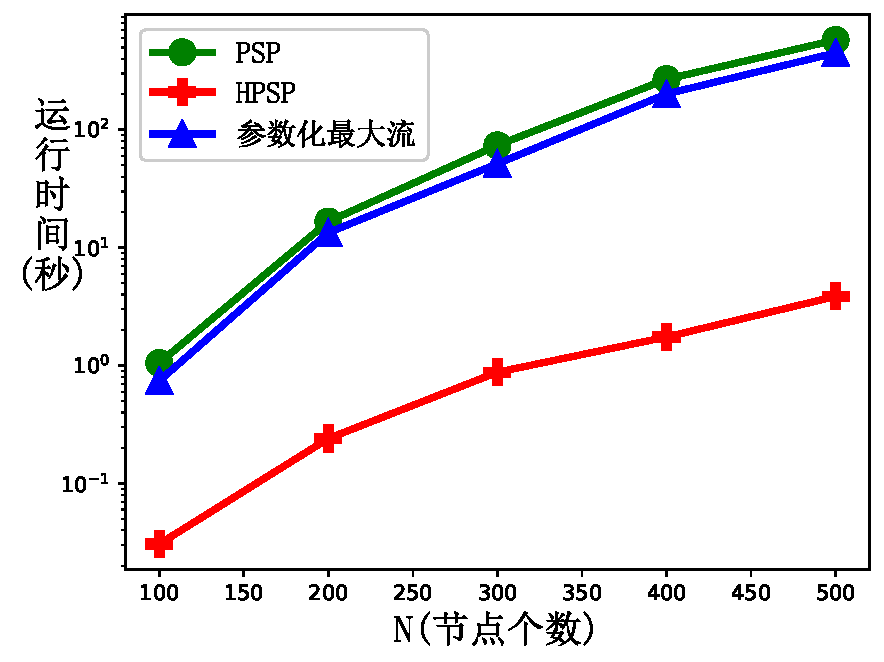
\includegraphics[width=\textwidth]{2019-08-26-gaussian.pdf}
	\end{subfigure}
	\begin{subfigure}{0.45\textwidth}
		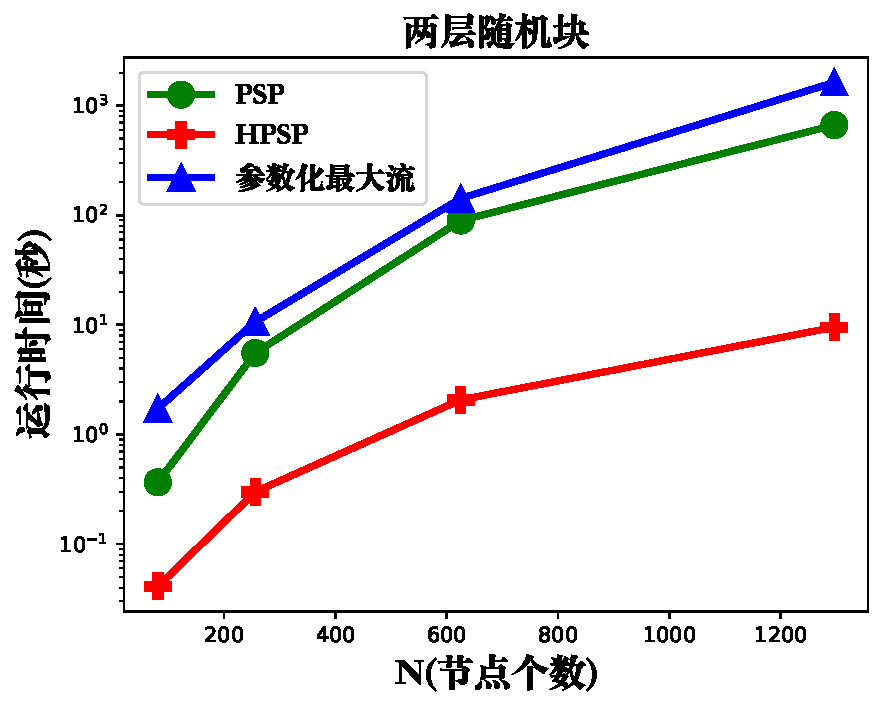
\includegraphics[width=\textwidth]{2019-09-19-two_level.pdf}
	\end{subfigure}
	\caption{
  不同PSP实现的速度比较}\label{fig:esc}
\end{figure}

另外我们注意到,
基于参数化最大流的
算法\citep{kolmogorov}在实践中表现不佳。
这可能与计算过程中构造中间图结构
和维护并发线程的额外成本有关。在实际实现中,
并发线程的创建和销毁的时间开销是不可忽略的,而这一部分
在复杂度理论分析中考虑。

\section{基于图分割的社群发现算法在异常值检测领域的应用}
异常值检测是对异常数据(称为异常值点)的识别,
这些异常数据不同于其他多数数据(称为正常值点)
\citep{grubbs1969procedures}。
在本节中,我们考虑将信息聚类算法用到异常值检测领域。

首先我们在理论层面探讨异常值检测背景下信息聚类的应用。
假设一个简单的情形,所有正常值点属于同一类别,
假设集合$B$达到式\eqref{eq:largest_threshold}中的
最大值,
我们认为$B$中的元素是正常值点,而$V\backslash B$ 是异常值点。

我们这里探讨的问题是, 假设有一个新的点$i'$加入到
现有的图 $G$ 中,如何判断它是正常值点还是异常值点。 
事实上,对于加入$i'$的图来说,
我们可以用PSP算法计算一个新的最大临界值
$\gamma'_N$,
并把它与 $\gamma_N$作比较。 由式\eqref{eq:largest_threshold}易得
$\gamma'_N \geq \gamma_N$。如果不等号严格成立,我们看到$i'$的作用是使得
多变量互信息的最大值增大了,说明$i'$与图$G$结合得更紧密,是正常值点,否则为异常值点。
实际上,我们不需要重新计算$\gamma'_N$就可以做出相同的判断,这个理论保证由下面的
定理给出
\begin{theorem}\label{thm:main_N}
  假设 $B$ 关于图$G$ 达到式\eqref{eq:largest_threshold}中的
  最大值,$\gamma_N, \gamma'_N$ 分别是图$G$加入新的点$i'$前、后的最大临界值,则有
\begin{equation}
\gamma'_N > \gamma_N \iff  \sum_{i \in B} w_{ii'} > \gamma_N 
\end{equation}
\end{theorem}
定理 \ref{thm:main_N} 给出了一种划分正常值点边界的方法,
假设图$G$的第$i$个点
对应一个高维空间的向量$x_i$,新加入的点对应的向量是$x$,
边的权值由rbf核给出,则边界曲线的方程为:
\begin{equation}\label{eq:sum_exp_gamma_N}
  \sum_{j \in B} \exp(-\gamma \norm{x - x_j}^2)= \gamma_N
\end{equation}

上述讨论假设了所有正常值点同属一个类别,
在实际应用中可能具有局限性。
下面我们在算法层面进行考虑,提出一个将信息
聚类的方法应用到异常值检测领域的方案。
假设在一个多分类问题中存在若干异常值点,
我们的目标是获得数据的一个分割,其形式为
$\{C_1, \dots, C_K, \{x_1\}, \dots, \{x_M\}\}$。
这里 $K$ 表示类别数 而 $M$ 表示异常值点的个数。
这两个参数在实际问题中通常是未知的,这里我们也做此假定,
我们使用的方法是基于 PSP 算法来获得该形式与$K, M$的值。

如果 $K$ 和 $M$ 较小, 使用式 \eqref{eq:PSP_structure}
的记法, 处理这种情况的一种经验性但合理的方法是找到一种划分。
$\P_{k-r}$ from  $\{\P_k, \P_{k-1}, \dots, \P_0\}$ 使得$K,M$都比较小。
对于此多目标优化问题,我们需要一个折中方案,即通过枚举法$r=1,2,\dots$ 求解下面的优化问题
\begin{align}\label{eq:outlier_detection_proposal}
& \min_{r\in Z^+} r \\
s.t.\, & f(r):=(r+1)\abs{\P_{k-r}} < n
\end{align}
在式\eqref{eq:outlier_detection_proposal}中,我们注意到函数
$f(0)=|\P_k|=n$ 和 $f(k)=k+1<n$ ,可知优化问题有解。

然后我们用 $\P_{k-r}$ 中元素个数大于1的集合来标记各类别中的正常值点,
元素个数小于1的集合为异常值点的集合。

如果需要预测新的观测值是否是异常值点, 
我们使用类似于式\eqref{eq:sum_exp_gamma_N}给出的边界方程判决规则。
假设 $\lambda_{k-r}$ 是$\P_{k-r}, \P_{k-r+1}$ 两个分割对应的
分界值并且图$G$边的权值是使用 rbf 核 来构建的,
那么边界曲线方程可以写成下面的形式:
\begin{equation}\label{eq:boundary_curve_multiple}
\sum_{j \in C_i} \exp(-\lambda \norm{x - x_j}^2)= \lambda_{k-r}, \textrm{ 其中 } \, C_i \in \P_{k-r} \textrm{且}\,  \abs{C_i} > 1
\end{equation}
注意到 $C_i$ 是其中一个类别,
并且 一共有 $K$ 个 边界曲线。
如果新的观测值落在所有这些边界曲线的外部,
那么我们将其归类为异常值点。


我们准备了三个人工数据集来验证我们提出的异常值检测算法。
第一个数据集是一个高斯斑点,其中一些噪声点均匀分布在一个正方形中。
第二个数据集是我们将 $(0,0)$ 这个点加入到
\ref{sec:data_clustering} 节所描述的有4个类别的
Gaussian 数据集里。
最后一个数据集是两个错开的半圆形状(或月牙形状),
并且其周围分布着一些
噪点。
构造相似图的权值我们采用 rbf 核,其 异常值检测
效果如图 \ref{fig:boundary} 所示。
从前三幅图可以看出,由式\eqref{eq:boundary_curve_multiple}
给出的边界曲线近似于正常值点的闭包曲线。
\begin{figure}[!ht]
	\centering
	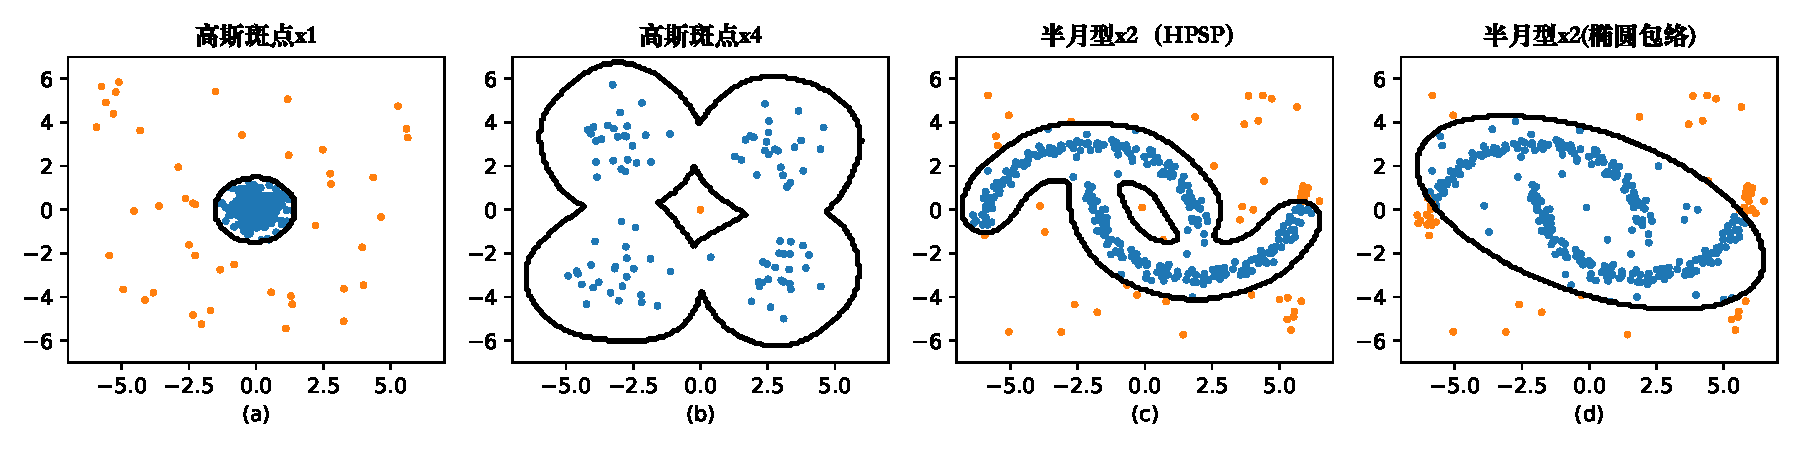
\includegraphics[width=\textwidth]{outlier_boundary_illustration.pdf}
	\caption{在人工生成的数据集上
  检测边界曲线的形状}
  \label{fig:boundary}
\end{figure}

另外我们也
在图 \ref{fig:boundary}.(d) 画出了椭圆包络(elliptic envelope \citep{rousseeuw1999fast} )方法的决策边界曲线。
由于后一种方法假设内部数据分布在凸区域,因此决策边界是椭圆形状,
因此不能很好地反映真实数据的分布。

下面我们针对不同的数据集比较本节提出的信息检测方法和其他常用的
异常值检测算法的性能。
我们使用 5 个数据集: Gaussian-blob, Moon, Lymphography
\cite{lazarevic2005feature}, Glass 和 Ionosphere \cite{keller2012hics}。 
前两个数据集如前所述是
人工生成的。
后三个数据集在异常值检测算法比较的文章中大量使用
\cite{campos2016evaluation}。
我们对比的方法包括
局部异常因子(local outlier factor \citep{Breunig}), 孤立森林(isolation forest \citep{if}), 
椭圆包络  和
一类支持向量机 (one class SVM \citep{svm})。 
我们使用TPR和TNR来衡量检测的整体性能。
正常值点被视为正样本。
TPR衡量的是正样本集合中正确检测的百分比,
而TNR衡量的是异常值点中正确检测的百分比。
通常而言,一种检测方法很难在这两个指标上都获得高分。
我们设法最大化TNR,同时控制每种方法的TPR$\geq 90\%$。
每个方法的超参数和相似度度量都经过了调优,TNR的最佳结果如表\ref{tab:odm}所示。我们可以看到,信息检测在 GaussianBlob,Moon 和
Lymphography 数据集上表现最好,与局部异常因子效果差不多,
但在 Glass 和  Ionosphere 两个数据集上性能有待提升。
\begin{table}
  \begin{adjustbox}{width=\columnwidth,center}
\begin{tabular}{cccccc}
  \hline
         TPR/TNR        &  GaussianBlob   &      Moon       &  Lymphography  &     Glass     &  Ionosphere   \\
  \hline
      信息检测    & 100\%/100\% & 97.4\%/100\%  & 97.9\%/100\% & 91.2\%/11.1\% & 90.7\%/48.4\% \\
      局部异常因子 & 100\%/100\% & 100\%/100\% & 98.6\%/83.3\%  & 96.6\%/22.2\% & 90.2\%/82.5\% \\
   孤立森林   & 100\%/100\% &  96.7\%/77.8\%  & 99.3\%/100\% & 89.8\%/11.1\% & 80.4\%/65.1\% \\
    椭圆包络   & 100\%/100\% &  91.3\%/42.2\%  & 93.0\%/83.3\%  & 94.6\%/0.0\%  & 93.3\%/88.1\% \\
     一类支持向量机     &  98.8\%/91.1\%  &  93.0\%/55.6\%  & 93.0\%/66.7\%  & 91.7\%/22.2\% & 83.1\%/69.0\% \\
  \hline
  \end{tabular}
\end{adjustbox}
\caption{不同异常值检测的算法比较}\label{tab:odm}
\end{table}

\section{本章小结}
在本章中,
我们考虑了信息聚类方法在图数据上的应用,
提出了基于图分割的信息聚类算法。该算法即求解
多个弱独立的随机变量的多变量互信息。
为实现图上的信息聚类,我们改进了一种计算图的主划分序列的有效算法,
用于推导聚类树的层次结构。
实证研究表明,基于图分割的信息聚类可以应用于数据聚类,社群发现以及异常值检测等多个领域,
在广泛的数据集上表现良好。
在有层次结构、类别数未知以及
含有异常值点的情况下,基于图分割的信息聚类具有更加明显的优势。
